\appendix
\section{Appendix}
\label{sec:Appendix}

  \subsection{Angular correction}

  Our straws don't actually measure U and V coordinates directly, but instead measure the distance of closest approach radii deriving from measured hit times. In order to utilize the minimization procedure on measured track parameters these radii must first be converted to U and V parameters, and similarly for the U and V errors. (Note that a future Kalman filter will not be subject to this disadvantage.) This is done in the calcMeasuredParams method at the bottom of the GeaneParamUtils class. These conversion corrections will be dependent on the angle of the track, so it's imporant to note that during each successive iteration, the ``measured'' parameters are adjusted by the latest ``predicted'' momenta. It was found that for the error correction, a simple straight line correction was sufficient for ideal results. For the position correction, it was found that a constant field correction for curved tracks was sufficient.

  To calculate these corrections, first the momentum perpendicular to the straw measurement axis can be ignored since it won't affect the U or V value. Because the positron tracks curve in only one direction through the tracker, one needs to calculate the correction depending on whether the track went to the left or right side of the wire. See Figure \ref{fig:angularCorrection} for a pictorial representation of the problem. The calculation of the right side correction follows, with the left side correction being calculated in a similar manner.

	\begin{figure}[]
	\caption{Shown here is a positron passing through a straw. The desire is to convert the measured parameter d into a U or V position, which can be done by approximating the particle trajectory as a circle in a constant magnetic field over the course of the straw and using trigonometry. Sizes and angles are exaggerated.}
	\centering
	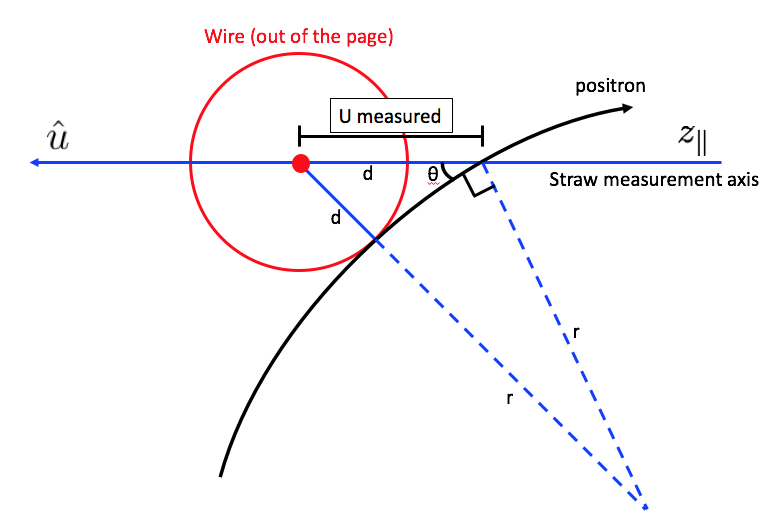
\includegraphics[width=1.0\textwidth]{angularCorrection}
	\label{fig:angularCorrection}
	\end{figure}

  To solve for the measured U (or V) value, we can use the equation:
	\begin{align}
		(r+d)^{2} = r^{2}+u^{2}-2ru\cos(90+\theta),
	\end{align}
  where the 90 degrees is approximate for large curvature of tracks. The angle $\theta$ can be determined from 
	\begin{align}
		\hat{z_{\parallel}} \cdot \hat{p_{\parallel}} = \cos{\theta}, \hspace{.1cm} \theta = \cos^{-1}{\frac{p_{\parallel}}{p}}, 
	\end{align}
  where $p_{\parallel}$ is the positron momentum parallel to the $z_{\parallel}$ axis at the wire plane and can be determined within the code. (The $z_{\parallel}$ axis simply stands for the axis perpendicular to the straw and parallel to the U measurement axis, but opposite in direction. At the end this calculated U value will simply be added or subtracted to the wire center U position depending on which side of the wire the positron travelled.) Using some trig identities and solving for u gives
	\begin{align}
		u = -r\sqrt{1-(\frac{p_{\parallel}}{p})^{2}} + \sqrt{d^{2} + 2dr + r^{2}(1-(\frac{p_{\parallel}}{p})^{2})},
	\end{align}
  for the right side correction, and 
	\begin{align}
		u = +r\sqrt{1-(\frac{p_{\parallel}}{p})^{2}} - \sqrt{d^{2} + 2dr + r^{2}(1-(\frac{p_{\parallel}}{p})^{2})},
	\end{align}
  for the left side correction. (Corrections to v are identical.) The radius of the particle circle can be calculated from the circular momentum and magnetic field at the predicted hit position. The straightline correction is done simply using the Pythagorean theorem in a simpler manner, with the correction to the errors then being
	\begin{align}
		\sigma_{uv}' = \frac{\sigma_{uv}}{\sqrt{1-(\frac{p_{\parallel}}{p})^{2}}}.
	\end{align}


\subsection{Matrix Transformation}
\label{sec:MatTransf}

  Transport matrices are accumulated as
      \begin{align} %\label{eq:nolabel}
        T_{mn} = T_{mk}T_{kn},
      \end{align}
  where the indices can stand for either plane numbers or step numbers, and converted by 
      \begin{align} %\label{eq:nolabel}
        T_{mn,s} = A_{m} T_{mn,f} A_{n}^{-1},
      \end{align}     
  where the indices s and f stand for the surface and free trajectory states respectively, and A is the Jacobian transformation from the free state to the surface state on a particular plane m or n. See \cite{jacob} for the calculation of these Jacobians. The error matrices in the surface state can be grabbed directly from the Geant code unlike the transport matrices, or if necessary can be converted as
      \begin{align} %\label{eq:nolabel}
        \sigma_{m,s} = A_{m} \sigma_{m,f} A_{m}^{-1}.
      \end{align}  



\subsection{GEANEArtRecord.hh} 
\begin{longtable}{|p{16cm}|}
% \scriptsize
\caption{GEANEArtRecord.hh active variables. This is subject to change. GEANEArtRecord contains vectors of variables on planes, as well as larger objects containing information about the whole track. Note that Eigen matrix objects cannot be stored into art data products. For this reason, and for minimal code changes, it was decided to add a data object for each Eigen member, made up of vectors with the word ``Data'' tagged at the end. The data objects are saved when creating GEANEArtRecords using a utils file. In analyzers accessing the GEANEArtRecords, these data objects are then swapped into the Eigen objects using the same utils file.}
 
\label{tab:artRecord}

% \begin{tabular}{|p{16cm}|}

  \\ \hline

enum GeaneHitSide \\ 
\textit{An enum for which side of the wire the track hit is guessed or calculated to have passed. Options are gLeft, gRight, gCenter, gNA\_side, and gUnknown. The first three are self explanatory, gNA\_side simply means there wasn't a hit, and gUnknown is used within the LR sequence checking part of the fitting code where any hits with said value or looped over to try and find the best choice.} 

  \\ \hline

art::Ptr \textless{} gm2strawtracker::TrackCandidateArtRecord \textgreater{} candidate \\
\textit{One track corresponding to one candidate corresponding to one GEANEArtRecord for the whole track.} \\ \hline

std::vector\textless{} art::Ptr\textless{} gm2truth::GhostDetectorArtRecord \textgreater{} \textgreater{} dummyPlaneHits \\
\textit{Associated dummy plane hits on planes aligned with straw wires, vector consists of hit dummy planes corresponding to hit wire planes (if a straw plane was skipped but that dummy plane was hit, it is not included in this vector. Vector has size N = num hits in straws that form the track +1 for the 0 plane.)} \\ \hline

int failureMode \\ 
\textit{Different failure modes for failed track reconstruction, 0 means it passed.} \\ \hline

double chi2 \\ 
\textit{Chi2 for whole track.} \\ \hline

std::vector\textless{}double\textgreater{} chi2Iterations \\
\textit{Chi2s for whole track for different iterations.} \\ \hline

std::vector\textless{}double\textgreater{} chi2Planes \\
\textit{Individual chi2s on each plane which add up to total chi2, vector consists of hit planes with size N.} \\ \hline

int numIterations \\
\textit{Number of iterations to converge.} \\ \hline

unsigned int dof \\
\textit{DoF of track = number of hit planes - 5 track parameters.} \\ \hline

double chi2DoF \\
\textit{chi2/dof} \\ \hline

double pValue \\
\textit{Fit pValue for whole track.} \\ \hline

double energyDiff \\
\textit{energy loss between first and last hit in track - from truth, for material characterizing} \\ \hline

std::vector\textless{}double\textgreater{} startingTrackParameters \\
\textit{Starting parameters for track: size 6, 3 position then 3 momentum, x y z px py pz, best starting parameters updated after each iteration, starting parameters x position defined before first hit.} \\ \hline

std::vector\textless{}double\textgreater{} startingTrackGuessOffsets \\
\textit{Size 10, x y z px py pz p 1/p pu/px pv/px offsets in different starting track parameters for plotting purposes.} \\ \hline

int trackNumPlanesHit \\ 
\textit{Total number of planes hit.} \\ \hline

int trackFirstPlaneHit \\ \hline

int trackLastPlaneHit \\ \hline

std::vector\textless{}int\textgreater{} trackPlanesHitList \\
\textit{List of hit planes, with missed planes excluded from the vector. Ex. 1 2 4 5 8 9} \\ \hline


std::vector\textless{}std::vector\textless{}double\textgreater{} \textgreater{} wireUVPositions \\
\textit{Wire center U and V postions, first vector is track param vector size 5 (0 1 2 unfilled, 3 is U, 4 is V), second vector is planenumber from 0 - 32  (formatted this way to align with other similar vectors - can probably be reduced.)} \\ \hline

std::vector\textless{}double\textgreater{} measuredDCAs \\
\textit{Vector of measured DCAs for hit planes, with size 33. Mainly to hold on to smearing values for now.} \\ \hline

std::vector\textless{}double\textgreater{} UVerrors \\
\textit{Vector of UV measurement errors for planes 0-32. Built in order to accomadate varying errors in the future.} \\ \hline

std::vector\textless{}double\textgreater{} planeXPositions \\
\textit{Vector of X postions of hit wire planes with size 33 (0 - 32), 0 plane being in front of the first module that was hit.} \\ \hline

std::vector\textless{}std::vector\textless{}double\textgreater{} \textgreater{} geaneMeasuredParameters \\
\textit{Measured GEANE parameters, first vector is param num 0 - 4, second vector is plane number 0 - 32, units are MeV mm. 1/P, Pu/Pz, Pv/Pz, U, V - only U or V is filled at the start of the GEANE fitting module.} \\ \hline

std::vector\textless{}std::vector\textless{}double\textgreater{} \textgreater{} geanePredictedParameters \\ 
\textit{Predicted GEANE parameters, first vector is param num 0 - 4, second vector is plane number 0 - 32, units are MeV mm. 1/P, Py/Px, Pz/Px, Y, Z - all params filled in tracing stage of GEANE fitting module - coord system has to be orthogonal - converted to UV locally in the fitting module.} \\ \hline

std::vector\textless{}GeaneHitSide>\textgreater{} geaneHitSides \\
\textit{Vector of GeaneHitSide enums with size 33 describing the sides of the wires that each hit of the track passed.}
 

std::vector\textless{}Eigen::MatrixXd\textgreater{} geaneTransportMatrices \\
std::vector\textless{}std::vector\textless{}double\textgreater{} \textgreater{} geaneTransportMatricesData \\ 
\textit{Units of GeV cm - transport matrices between planes tracked to in GEANE fitting module, 5x5 objects. Vector has size 33.} \\ \hline

std::vector\textless{}Eigen::MatrixXd\textgreater{} geaneErrorMatrices \\ 
std::vector\textless{}std::vector\textless{}double\textgreater{} \textgreater{} geaneErrorMatricesData \\ 
\textit{Error matrices on tracked to planes, units GeV cm, size 33.} \\ \hline

Eigen::MatrixXd covarianceTotalInverse \\
std::vector\textless{}double\textgreater{} covarianceTotalInverseData \\
\textit{5x5 inverse of total covariance matrix for track. Diagonals represent errors in 5 track paramaters on plane 0.} \\ \hline

std::vector\textless{}Eigen::VectorXd\textgreater{} paramPredictedInUVEigen \\ 
std::vector\textless{}std::vector\textless{}double\textgreater{} \textgreater{} paramPredictedInUVEigenData \\ 
\textit{Predicted parameters in UV space as an eigen object (converted from geanePredictedParameters above) for calculation convenience and some LR information storage. Order of vectors is switched here, first is planenum, second is paramnum, units are MeV mm.} \\ \hline

\textit{Objects below here are full track objects with larger sizes, held on to for fast sequence checking. Units GeV cm.} \\ \hline

std::vector\textless{}Eigen::MatrixXd\textgreater{} extendedTransportMatrixBegToEnd \\
std::vector\textless{}std::vector\textless{}double\textgreater{} \textgreater{} extendedTransportMatrixBegToEndData \\ 
\textit{Accumulated/combined transport matrices from starting plane to all following planes.} \\ \hline

Eigen::MatrixXd extendedCombinedTransportMatricesTranspose \\
std::vector\textless{}double\textgreater{} extendedCombinedTransportMatricesTransposeData \\
\textit{Transpose of larger eigen object composed of above begtoend transport matrices.} \\ \hline

Eigen::MatrixXd extendedReducedMatrix \\
std::vector\textless{}double\textgreater{} extendedReducedMatrixData \\ 
\textit{Total error correlation matrix, reduced to size NxN (N = num planes hit).} \\ \hline

Eigen::MatrixXd extendedReducedMatrixInverse \\ 
std::vector\textless{}double\textgreater{} extendedReducedMatrixInverseData \\
\textit{Inverse of above saved once for LR checking.} \\ \hline

Eigen::MatrixXd extendedModifiedReducedMatrix \\ 
std::vector\textless{}double\textgreater{} extendedModifiedReducedMatrixData \\
\textit{Reduced matrix from above that's going to be modified into a hybrid error matrix separately for U and V fits but that needs to be held onto for all sequences.} \\ \hline



std::vector\textless{}int\textgreater{} hitSidesCorrect \\
\textit{Vector of ints as to whether the sides that the track fitting guessed/calculated were correct or not - only available when truth is available. 1 for correct, 0 for no hit, and -1 for incorrect. Almost certainly temporary.} \\ \hline


  \hline

% \end{tabular}
\end{longtable}


